\section{Escenario y Análisis}\label{sec:experiments}
\subsection{Escenario modelado}

\begin{figure}[tpb]
    \centering
    \begin{subfigure}{0.8\textwidth}
        \centering
        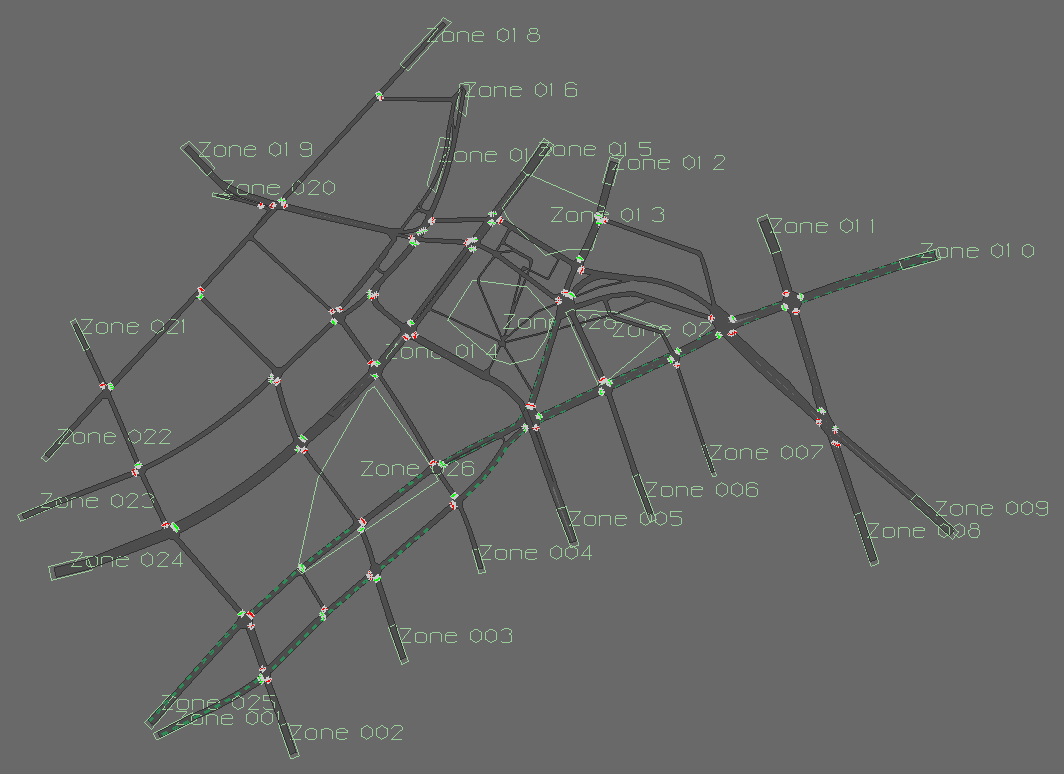
\includegraphics[width=\linewidth]{figuras/costanera.png}
        \caption{Mapa en Paramics del escenario simulado.}
    \end{subfigure}\\
    \begin{subfigure}{0.8\textwidth}
        \centering
        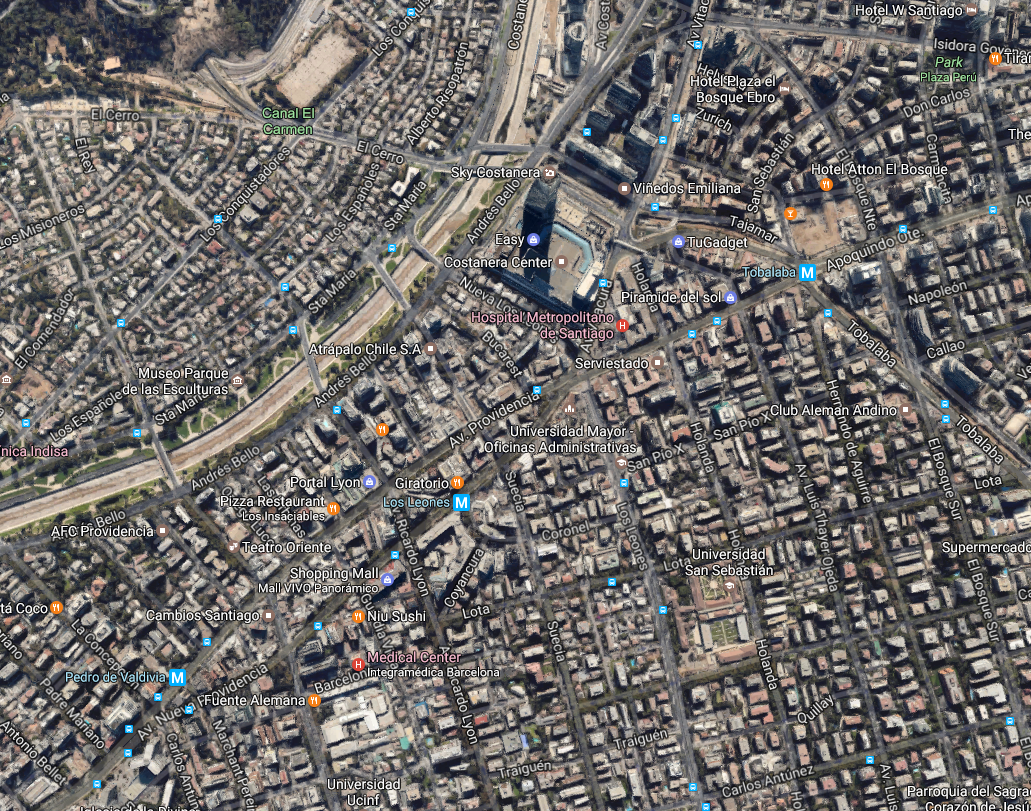
\includegraphics[width=\linewidth]{figuras/costanera_maps.png}
        \caption{Escenario simulado en la ``vida real'', Google Maps.}
    \end{subfigure}
    \caption{Escenario modelado, Paramics vs. ``vida real''.}
    \label{fig:costanera}
\end{figure}

Como escenario de transporte para la validación del \emph{framework} se utilizó un modelo de un sector de la ciudad de Santiago de Chile, el cual consiste en una simulación detallada del flujo vehicular en la comuna de Providencia. Este modelo fue creado en 2010 por Víctor Zúñiga para el desarrollo de su memoria de grado \autocite{zuniga}, y simula el impacto sobre el sector entre las avenidas Providencia, Tobalaba, Andrés Bello y Santa María proyectado en ese entonces por la construcción de un nuevo centro comercial (ver figura \ref{fig:costanera}).

Sobre este escenario vehicular se construyó un modelo de ITS, utilizando el \emph{plugin} desarrollado y el \emph{framework} VEINS en OMNeT++. Este consistió en un escenario en que un vehículo sufre un desperfecto en una cierta calle de la simulación y emite \emph{beacons} de advertencia en \emph{broadcast} a todos los demás vehículos que se encuentran dentro del alcance de la transmisión. A aquellos vehículos que reciben un \emph{beacon}, y que se puede predecir ingresarán a a la calle en que se encuentra el vehículo averiado, se les modifica luego su ruta mediante VEINS y TraCI.

De manera más detallada, el escenario funciona de la siguiente manera:

\begin{enumerate}
    \item Al iniciarse el \emph{framework}, OMNeT++ (utilizando VEINS) inicializa una conexión TraCI con el \emph{plugin} en Paramics.
    \item Por cada vehículo que ingresa a la red de transporte, OMNeT++ crea un módulo dotado de lógica y capacidades comunicaciones en su simulación de red, y asocia el movimiento de este módulo al vehículo en Paramics. En adelante, se entenderá por ``vehículo'' el par consistente en el vehículo en Paramics y su módulo asociado en OMNeT++.
    \item Periódicamente se verifica la posición de cada vehículo, y al detectar el primero en ingresar a la calle del ``accidente'', este es detenido. La calle en cuestión para esta simulación fue el arco ``40:5'', el cual corresponde a Avenida Vitacura, frente al centro comercial. El vehículo además se colorea rojo para su fácil identificación.
    \item El módulo OMNeT++ del vehículo accidentado emite luego, cada 5 segundos, un mensaje WAVE \autocite{80211wave} en \emph{broadcast}.
    \item Aquellos vehículos que reciban el \emph{beacon} de emergencia, se encuentren en alguna de las calles aledañas al accidente y que tengan un destino que probablemente los haga pasar por la calle afectada, cambian su ruta a utilizar el arco ``40:7'', correspondiente a la calle Holanda, entre Avda. Vitacura y Avda. Providencia. Además, se cambia su color a púrpura para visualizarlos de manera más fácil en Paramics.
\end{enumerate}

Esta simulación dura un total de \textbf{15 minutos de tiempo \emph{simulado}}, y se ejecutó con múltiples configuraciones del sistema de transporte y del sistema de comunicaciones, las cuales se verán a continuación en las secciones \ref{sec:results:performance} y \ref{sec:results:vehicular}. Las especificaciones técnicas del equipo en donde se realizaron estos experimentos pueden observarse en la tabla \ref{table:systemspecs}.

\begin{table}[tpb]
    \centering
    \begin{tabular}{@{}ll@{}}
        \toprule
        Sistema Operativo     & Windows 10 v.10.0.14393         \\
        Procesador            & Intel Core i7 4720HQ @ 2.60 GHz \\
        N$^{o}$ de Núcleos / Threads & 4 núcleos / 8 threads\\
        Arquitectura          & x86\_64                         \\
        RAM                   & 12 GB DDR3L 1600 MHz            \\
        Tarjeta de Video      & NVIDIA GeForce GTX 960M         \\
        Memoria Video         & 2 GB GDDR5                      \\ \bottomrule
    \end{tabular}
    \caption{Especificaciones técnicas del entorno de simulación.}
    \label{table:systemspecs}
\end{table}

Las mediciones realizadas se enfocaron a probar el funcionamiento del \emph{framework} en dos categorías de análisis; \textbf{eficiencia computacional} de la implementación e \textbf{impacto sobre el modelo de transporte}. De esta manera se pretende demostrar que PVEINS es una opción viable para la investigación en Sistemas Inteligentes de Transporte, tanto en términos de los recursos que utiliza el \emph{framework} para la ejecución de las simulaciones como en términos de la validez de los resultados obtenidos.

Los resultados obtenidos de cada simulación fuero exportados desde OMNeT++ a archivos CSV, los cuales luego se analizaron utilizando Python 3.6.
Se utilizaron las librerías Pandas \autocite{pandas}, para el manejo de los datos de manera eficiente, Numpy \autocite{numpy}, para cálculos, y Matplotlib \autocite{matplotlib} y matplotlib2tikz \autocite{matplotlib2tikz} para la generación de gráficos que permitiesen analizar los datos de manera más efectiva e intuitiva.

